\chapter{Experiment}

This report has focused primarily on the numerical study of transport properties in complex networks using simulation. However, the long-term goal of this project is to experimentally realise complex nanophotonic networks as light engineering platforms. The experimental component of this project is still in its preliminary stages, therefore we will only briefly describe the setup and some early progress.

\section{Setup and equipment}

We study the classical transport properties of silicon nitride networks by sending in pulsed broadband (supercontinuum) laser light generated by a SuperK Compact laser (NKT Photonics). We filter out most of the power in the IR range, and further reduce the laser power using neutral density filters (Thorlabs). The network samples (design shown in Fig.\ref{fig:chip_design} were designed by Michele Gaio and fabricated by Fred Gardes, and have grating couplers optimised for $633nm$ and $785nm$. Light is coupled into and out of the samples via fibres (single-mode S630-HP for input and multi-mode FG105 for output, both Thorlabs), mounted on custom fibre stages shown in Fig.\ref{fig:exp_setup}. An objective mounted above as well as a camera on the side of the sample stage allow us to visually align the fibres and gratings.
\begin{figure}[htp]
  \centering
    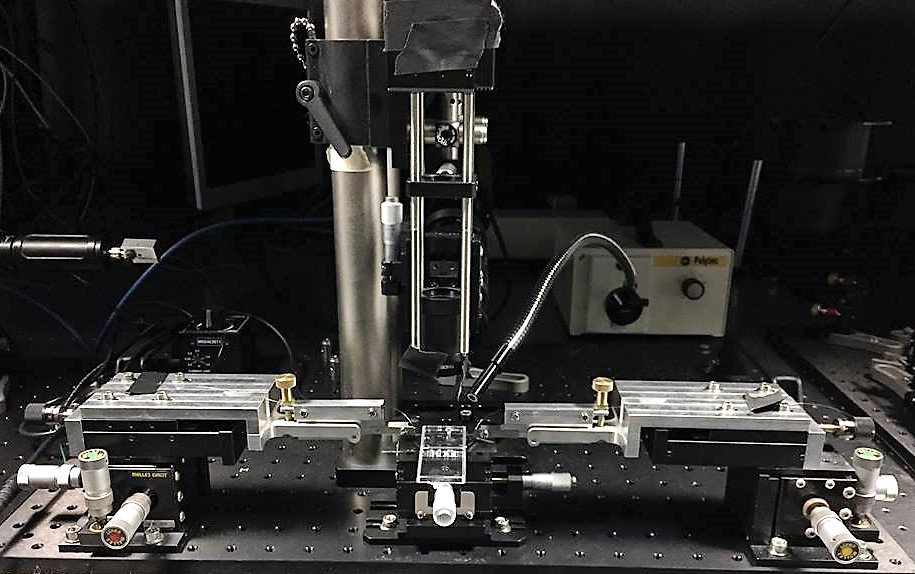
\includegraphics[width=0.65\textwidth]{ch4/fig4/exp_setup.jpg}
    \caption{Experimental setup. From left to right, we see the output fibre stage (connected to the spectrometer), the sample stage with an objective above, the input fibre stage (connected to a supercontinuum laser).} 
    \label{fig:exp_setup}
\end{figure}

\begin{figure}[hbp]
  \centering
    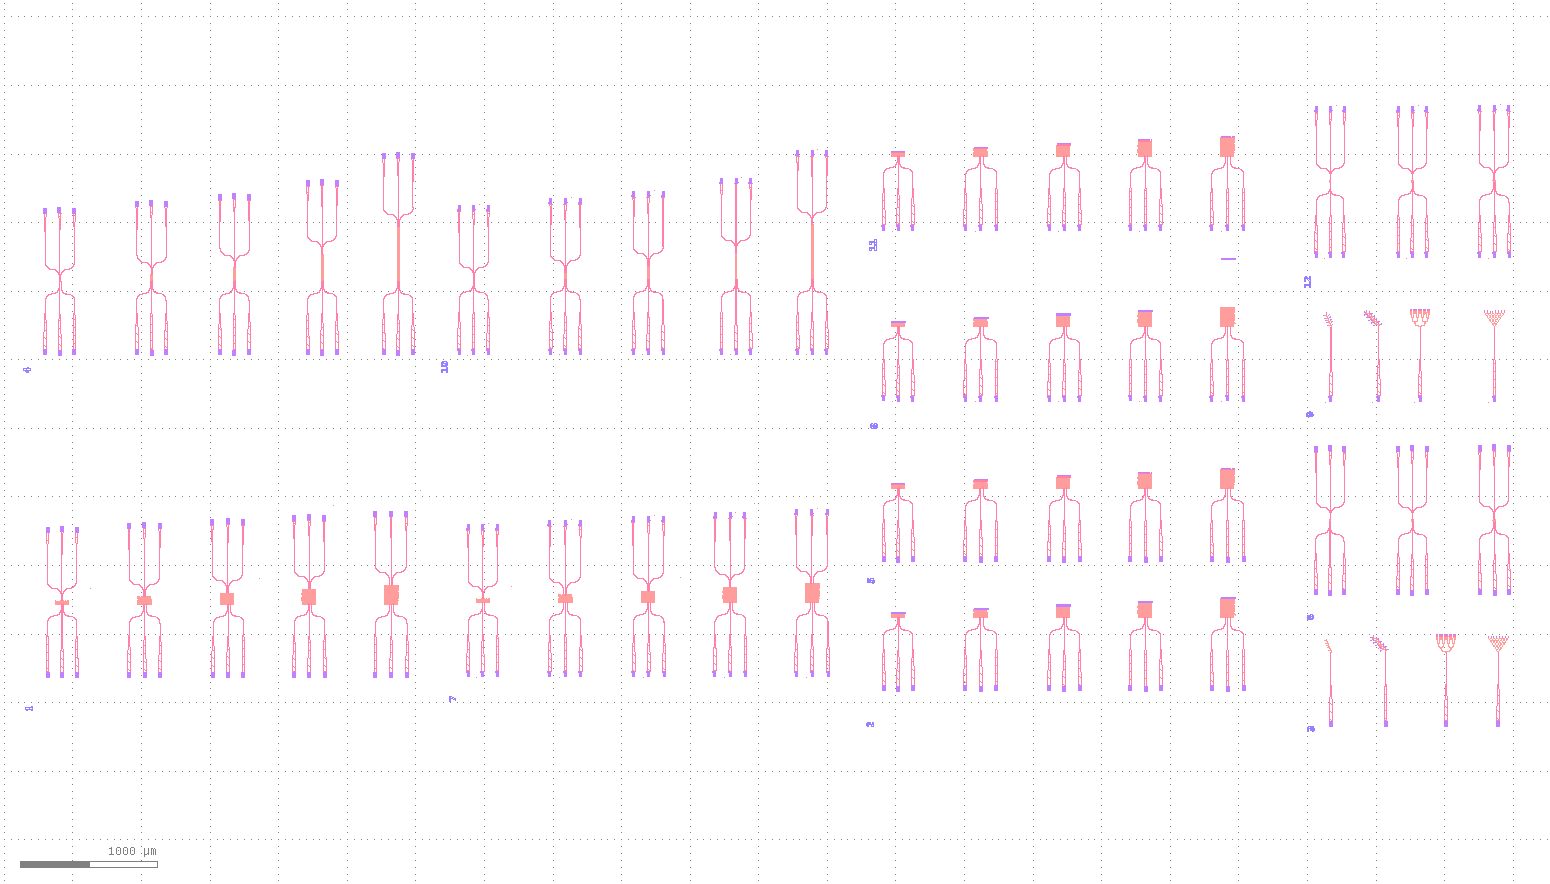
\includegraphics[width=0.8\textwidth]{ch4/fig4/chip_design.png}
    \caption{Sample design by Michele Gaio. The chip contains Voronoi networks of various sizes, as well as straight waveguides and tree-shaped networks.} 
    \label{fig:chip_design}
\end{figure}

\section{Preliminary measurements}
We are able to achieve coupling to the network samples (Fig.\ref{fig:coupling}) and measure output power spectra. However, the measurements are not reliable as the spectra are very sensitive to the position of the input fibre. 

\begin{figure}[h]
  \centering
    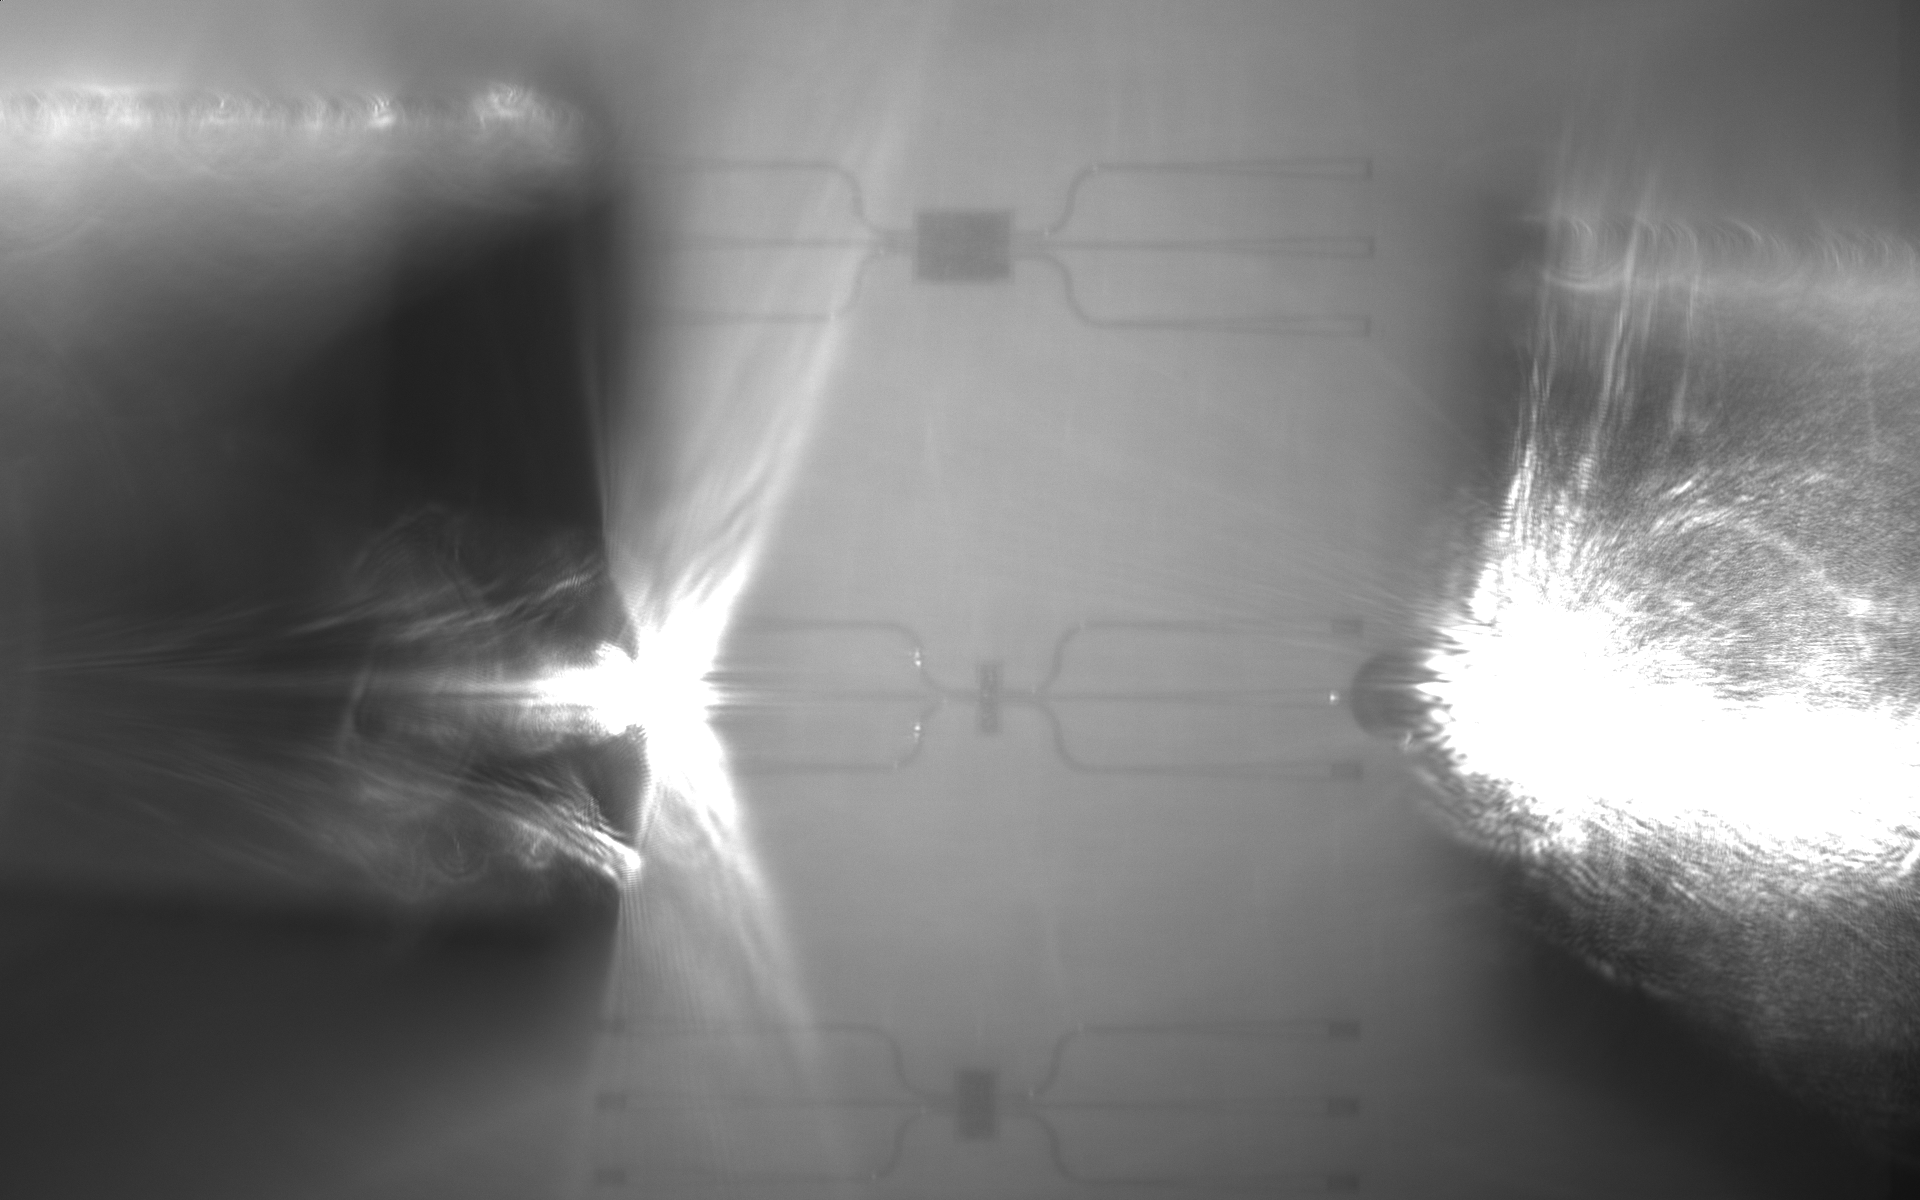
\includegraphics[width=0.5\textwidth]{ch4/fig4/785N1_coupling_top.png}    
    \caption{Coupling of light through a network sample; the bright dot on the right is light scattered from the output grating.} 
    \label{fig:coupling}
\end{figure}


\begin{figure}[hb]
  \centering
    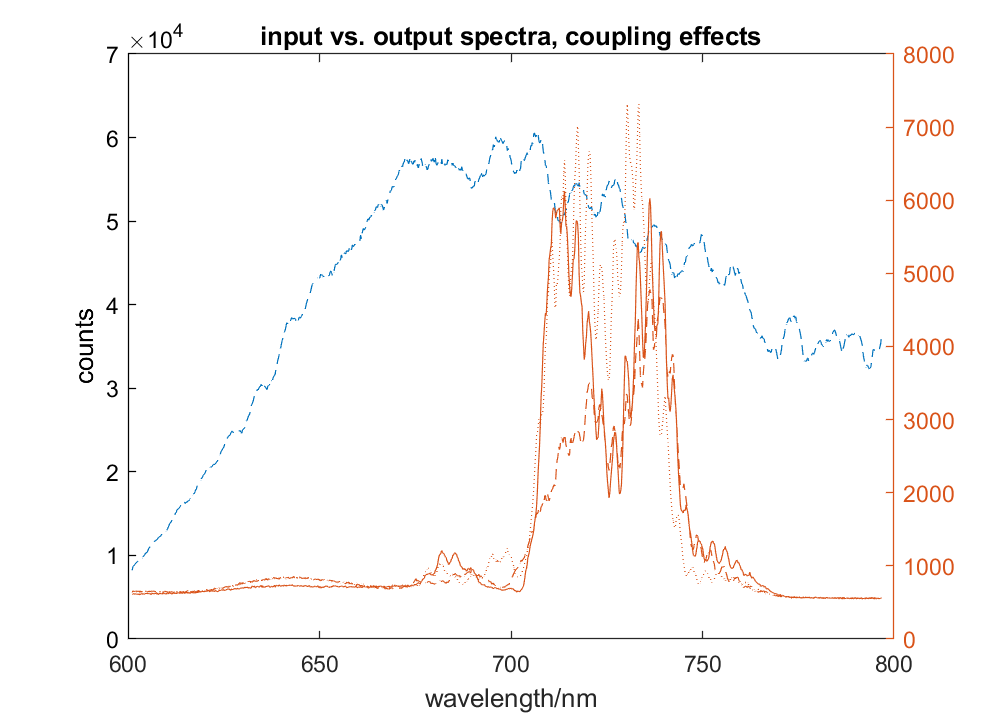
\includegraphics[width=0.7\textwidth]{ch4/fig4/specdata.png}
    \caption{Input supercontinuum spectrum (blue) plotted against three different output spectra (orange). The outputs are all measured with the exact same experimental configuration and on the same network, except the position of the input fibre is slightly altered.} 
    \label{fig:specdata}
\end{figure}


